\begin{figure}[tb]
\centering
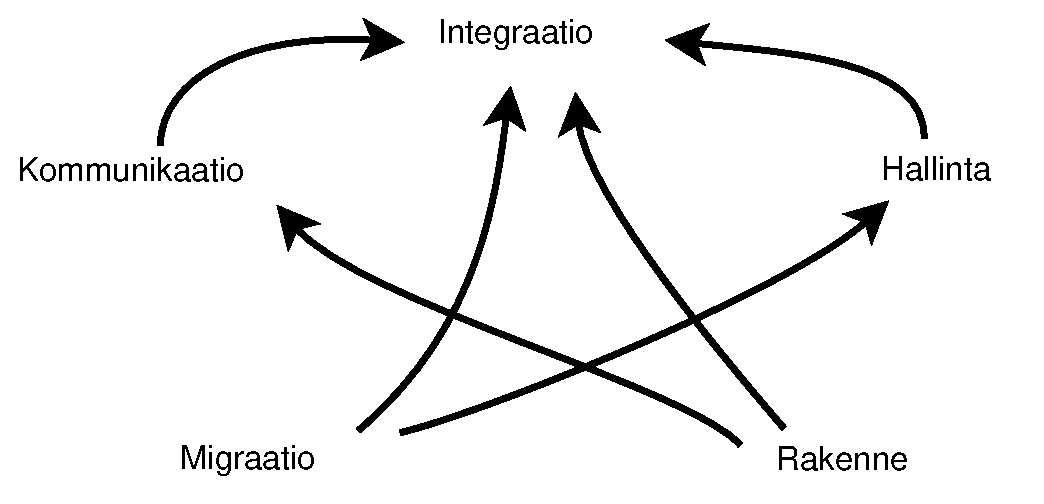
\includegraphics[scale=0.5]{riippuvuudet.eps}
\caption{Reuna-arkkitehtuurien ominaisuuksien yleiset riippuvuudet} \label{fig:riippuvuudet}
\end{figure}

\subsection{Vertailu}
Seuraavaksi käydään läpi edellä esitettyjen reuna-arkkitehtuuriehdotuksien ominaisuuksia ja käsitellään niiden vaikutuksia itse toteutettavaan järjestelmään.
Kunkin arkkitehtuuriehdotuksen ominaisuusjoukko ohjaa toteutusta erilaisiin ratkaisuihin. Taulukoon \ref{table:features} on tiivistetysti koottu kunkin arkkitehtuuriratkaisun ominaisuudet.
Lopuksi käsitellään reuna-arkkitehtuurien yhteneväisyyksiä ja eroja ETSI:n MEC spesifikaation kanssa.

On tärkeää huomata että käsiteltyjen ominaisuuksien välillä on riippuvuksia. Tämän seurauksena jonkin ominaisuuden toteuttaminen tietyllä tavalla saattaa estää tai rajoittaa joidenkin toiminnallisuuksien toteuttamista. 


Reuna-arkkitehtuurien keskeisin ominaisuus on tapa jolla järjestelmä integroituu osaksi mobiiliverkkoa. Kaikki muut ominaisuudet vaikuttavat olevan riippuvaisia tästä.
Kuvassa \ref{fig:riippuvuudet} on esitetty ominaisuuksien väliset riippuvuudet.
Rakenne on tyypiltään implisiittinen ominaisuus. Se ei siis pääsääntöisesti ole reuna-arkkitehtuurin määrittelemä, vaan sen toteutus on riippuvainen reuna-arkkitehtuurin muista ominaisuuksista.

Kappaleessa \ref{integraatio} esiteltyjen integraatiotyyppien jaon mukaan SCC ja CONCERT edustavat suoraa integraatiota, SMORE ja MobiScud edustavat läpinäkyvää integraatiota ja FMC edustaa epäsuoraa integraatiota.

SCC liittyy mobiiliverkon toimintoihin niin sanotusti natiivien yhteyksien avulla. Se edellyttää uusia rajapintoja mobiiliverkon nykyisiin komponentteihin. Tavoitteena on SCC:n hallinnollisten tarpeiden täyttämiseen. Lisäksi SCC edellyttää reunaresurssien integrointia osaksi tukiasemaa. 
Tukiasemaan sidottujen reunaresurssien vuoksi SCC:n rakenne on litteä. 
SCC:n mukaan uudistetun tukiaseman, eli SCeNBce:n, tehtäviin kuuluu reunapalveluille tarkoitetun tietoliikenteen ohjaaminen. Tämä tarkoittaa että SCeNBce monitoroi tietoliikennettä ja ohjaa esimerkiksi kohde IP:n perusteella reunapalvelulle tarkoitetut paketit.

CONCERT on toinen suoran integraation reunajärjestelmä. Ehdotuksen tavoitteena on NFV:n laajamittainen käyttöönotto, jonka seurauksena mobiiliverkon ja reunajärjestelmä voisivat jakaa laskentaresursseja. Järjestelmä rakentuu kolmeen kerrokseen hierarkisesti sijoitettujen resurssien varaan. Nämä resurssit ovat reunalaskennan ja mobiiliverkon toiminnallisuuksien käytettävissä. 
Mobiiliverkon ja reunalaskennan hallinnolliset toimet on yhdistetty Conductor nimiselle entiteetille. Conductor sisältää useita alitoimintoja joiden tehtäviin kuuluu muun muassa resurssien jakaminen kullekkin toiminnallisuudelle. CONCERT ottaa hallinnollisiin tehtäviin kantaa ainoastaan yleisellä tasolla ja yksityiskohdat jätetään avoimeksi. Oletettavaa on että CONCERT:ssa mobiiliverkon ja reunajärjestelmän reititys tapahtuu samassa kontekstissa, jolloin järjestelmä ei vaadi erillistä toiminnallisuutta reunasolmuille suuntautuvan tietoliikenteen ohjaamiseen. 

MobiScud ja SMORE edustavat läpinäkyvää integraatiota.
SDN-kerros eNodeB ja EPC:n komponenttien välillä mahdollistaa tietoliikenteen monitoroinnin sekä ohjaamisen.
SDN-kerros mahdollistaa mobiiliverkon nykyisten toimintojen säilyttämisen ennallaan.
Koska tietoliikenne reunaresursseille ohjataan SDN-kerroksen sisällä, reunasolmujen sijoittelu ei ole suoranaisesti riippuvaista mobiiliverkosta.  
Teoriassa reunasolmujen sijoittelu on täysin vapaa. 
SMORE ja MobiScud ehdottavat toisistaan poikkeavaa sijaintia reunasolmuille. SMORE:ssa yhdelle reunasolmulle klusteroidaan suuri joukko tukiasemia, kun taas MobiScud ehdottaa reunasolmujen sijoittelua yksittäisten tukiasemien yhteyteen.
Tämä tarkoittaa että järjestelmät eroavat yksittäiseen reunasolmuun sijoitettujen laskentaresurssien määrältä huomattavasti.
SMORE:n tapauksessa yhden reunasolmun vastuualueeksi oletetaan niin suuri joukko tukiasemia, että laskennan siirrolle ei ole tarvetta, eli järjestelmä ei toteuta live migraatiota.
MobiScud puolestaan hajautetummilla resursseillaan edellyttää reunalaskennan siirtoa ja ehdottaakin sille toiminnallisuutta.
SMORE:n ja MobiScud:n yhteisenä ominaisuutena on mekaniikka, jolla tietoliikenne ohjataan reunasolmuille siten että se ei vaikuta mobiiliverkon toimintaan.
Molemmissa ratkaisuissa SDN-kerros sisältää toiminnallisuuden, joka haarauttaa reunasolmuille tarkoitettua liikennettä monitoroimalla mobiiliverkon GTP liikennettä.
Tarpeen mukaan GTP tunneloitujen pakettien GTP paketointi puretaan ja välitetään SDN-kerroksen sisällä reunasolmulle. 
Samaa monitorointitoiminnallisuutta käytetään molemmissa ratkaisuissa myös mobiiliverkon kontrollitason seuraamiseen, joka mahdollistaa mobiiliverkon tapahtumiin reagoinnin.
MobiScud perustaa reunalaskentaan siirtoon liittyvät päätökset näihin mobiiliverkon tapahtumien kautta saatuihin tietoihin.
%
%Koska SDN-kerros sijaitsee eNodeB:n ja EPC:n välillä joudutaan asiakaslaitteen ja reunasolmun välistä liikennettä muokkaamaan. Kyseisellä välillä tietoliikenne on GTP tunneloitua.
%Riippuen onko paketti menossa reunasolmulle vai tulossa reunasolmulta, joudutaan tunnelointi purkamaan tai paketoimaan. Tämä saattaa johtaa merkittävään viiveeseen yhdessä monitoroinnin kanssa.
%MobiScudissa SDN-kerros sijaitsee eNodeB:n välittömässä läheisyydessä, kun taas SMORE:ssa sen oletetaan sijaitsevan useamman eNodeB:n yhteyspisteessä. 

Ainoa epäsuoraa integraatiota edustava ratkaisu on FMC.
FMC:n tavoitteena on viedä mobiiliverkon yhteydet nopeammin ulkoverkossa sijaitseville palvelinresursseille. Mobiiliverkon ulkopuolelle sijoitetut resurssit mahdollistavat sen että reunajärjestelmää voi ylläpitää jokin ulkoinen taho.
FMC ei siis suoranaisesti ota kantaa tapaan jolla reunaresurssit on järjestetty. Mutta on perusteltua olettaa että ne sijaitsisivat mobiiliverkon P-GW komponenttien läheisyydessä.
FMC:n tapa mahdollistaa reunapalvelun ja asiakaslaitteen välinen kommunikaatio perustuu sessiotunnistesiin. Se mahdollistaa asiakaslaitteen ja reunpalvelun IP-osoitteiden vaihtumisen, ilman että viitteet asiakaslaitteen ja reunapalvelun välillä katkeavat. Järjestelmä ei siis edellytä tavallisesta poikkeavaa mekaniikkaa tietoliikenteen reitittämiseksi. Ainoa edellytys on asiakaslaitteen sovellukseen sekä reunapalvelun toiminnallisuuden ohjelmallisen toimijan joka huolehtii yhteyksien varmistamisesta sessiotunnisteiden avulla.

Myös hallinnollisten toimien toteuttaminen on osittain riippuvaista integraatiosta. Suoran integraation järjestelmissä hallinnollisella entiteetillä on oma rajapinta mobiiliverkon toimintojen kanssa. 
Toisaalta se edellyttää olemassa olevaan järjestelmään rajapinnan toteuttamisen, mutta lisäksi tarjoaa helpon keinon tehdä hallinnollisia toimia mobiiliverkon sisällä. 
Läpinäkyvässä järjestelmässä hallinnollinen entiteetti on riippuvainen mobiiliverkon viestien monitoroinnin kautta saatavasta tiedosta. 
MobiScud ja SMORE tarkkailevat SDN-kerroksen avulla mobiiliverkon kontrollitason viestintää. 
Vaikka läpinäkyvät integraatiot ovat loogisesti erillään mobiiliverkosta, edellyttävät ne pääsyä mobiiliverkon sisäisiin tietoliikenneväyliin.
Todennäköisintä onkin siis että järjestelmää ylläpitää mobiiliverkon operaattori eikä ulkoinen taho. 
Epäsuoraa integraatiota edustavassa FMC:ssä hallinnolliset toiminnot edellyttävät tietoja mobiiliverkosta. Tieto on tyypiltään staattista, joten aktiivista tiedosiirtoa mobiiliverkon ja FMC:n välille ei tarvita.
Edellytyksenä on esimerkiksi taulukko, josta voidaan lukea asiakaslaitteen IP-osoittetta vastaava fyysinen alue tai P-GW:n sijainti. Tämä mahdollistaa FMC:n ohjata asiakaslaitteen yhteys lähimmälle palvelinsalille.

\subsubsection*{Yhteensoppivuus ETSI MEC vaatimuksiin}
%Reuna-arkkitehtuurien ominaisuuksien vertailu aloitetaan live migraatiosta.
%\par
%Live migraatio on toiminnallisuuksista se joka mahdollistaa suurempien palvelukokonaisuuksien siirtämisen reunajärjestelmässä. Syitä reunalaskennan siirtämiselle voi olla useita ja ehkä yleisin pinnalle noussut syy on asiakaslaitteen liikkuminen verkossa. Muita syitä live migraatiolle voi olla esimerkiksi laskennan siirtäminen enemmän resursseja sisältävälle reunapalvelulle tai ylikuormituksen välttäminen nykyisellä reunasolmulla.
%%migraatio edellyttää reunasolmujen olemista samalla palveluntarjoajalla.
%
%Live migraatio toiminnallisuuden puuttumisen voi tulkita ainakin kahdella tavalla. Joko se tarkoittaa, että reunalaskenta on muodoltaa etälaskentaa, joka on niin hienojakoista, että migraatiolle ei ole tarvetta. Tällöin etälaskenta rajoittuu pieniin työyksiköihin joista odotetaan välitöntä tulosta asiakaslaitteelle. 
%Toinen vaihtoehto on että tarjolla olevat reunasovellukset ovat tyypiltään yleiskäyttöisiä, esimerkiksi pelipalvelimia.
%
%Lähes kaikki reuna-arkkitehtuurit tiedostivat tarpeen live migraatiolle. Ainoastaan SCC ei sisältänyt edes mainintaa reunasovelluksien siirtelystä reunasolmulta toiselle.
%
%
%\par
%Reuna-arkkitehtuurin kommunikaatio
%
%\par
%Reuna-arkkitehtuurin 
%

% Taulukko toiminnoista
\begin{landscape}
    \noindent
\begin{table}[!ht]
\caption{Reunalaskenta-arkkitehtuurien ominaisuudet tiivistetysti}
\label{table:features}
\begin{tabularx}{ \linewidth }{ | c | c | c | p{3cm} | c | p{5cm} | }
\hline 
 \textbf{Ominaisuus} & \textbf{Integraatio} & \textbf{Rakenne} & \textbf{Migraatio} & \textbf{Hallinta} & \textbf{Kommunikaatio} \\ 
\hline 
 FMC & Epäsuora & Vapaa & Palveluiden siirto ulkopuolisten salien välillä & FMC Controller & Tavalliset reitityksen, palveluiden ja asiakaslaitteen yhdistämiseen erillinen sessiotunniste \\ 
\hline 
 SMORE & Läpinäkyvä & Vapaa & Ei sisällä & SMORE Controller & SDN monitori ja reititys \\ 
\hline 
MobiScud & Läpinäkyvä & Vapaa & Live migraatio & MobiScud Controller & SDN monitori ja reititys\\ 
\hline 
SCC & Suora & Litteä & Live migraatio & SCM & Monitori ja reititys tukiasemassa \\ 
\hline 
CONCERT & Suora & Hierarkinen & Live migraatio & Conductor & SDN reititys mobiiliverkossa \\ 
\hline 
\end{tabularx} 
\end{table}
\end{landscape}